\documentclass[twoside]{book}

% Packages required by doxygen
\usepackage{fixltx2e}
\usepackage{calc}
\usepackage{doxygen}
\usepackage[export]{adjustbox} % also loads graphicx
\usepackage{graphicx}
\usepackage[utf8]{inputenc}
\usepackage{makeidx}
\usepackage{multicol}
\usepackage{multirow}
\PassOptionsToPackage{warn}{textcomp}
\usepackage{textcomp}
\usepackage[nointegrals]{wasysym}
\usepackage[table]{xcolor}

% Font selection
\usepackage[T1]{fontenc}
\usepackage[scaled=.90]{helvet}
\usepackage{courier}
\usepackage{amssymb}
\usepackage{sectsty}
\renewcommand{\familydefault}{\sfdefault}
\allsectionsfont{%
  \fontseries{bc}\selectfont%
  \color{darkgray}%
}
\renewcommand{\DoxyLabelFont}{%
  \fontseries{bc}\selectfont%
  \color{darkgray}%
}
\newcommand{\+}{\discretionary{\mbox{\scriptsize$\hookleftarrow$}}{}{}}

% Page & text layout
\usepackage{geometry}
\geometry{%
  a4paper,%
  top=2.5cm,%
  bottom=2.5cm,%
  left=2.5cm,%
  right=2.5cm%
}
\tolerance=750
\hfuzz=15pt
\hbadness=750
\setlength{\emergencystretch}{15pt}
\setlength{\parindent}{0cm}
\setlength{\parskip}{3ex plus 2ex minus 2ex}
\makeatletter
\renewcommand{\paragraph}{%
  \@startsection{paragraph}{4}{0ex}{-1.0ex}{1.0ex}{%
    \normalfont\normalsize\bfseries\SS@parafont%
  }%
}
\renewcommand{\subparagraph}{%
  \@startsection{subparagraph}{5}{0ex}{-1.0ex}{1.0ex}{%
    \normalfont\normalsize\bfseries\SS@subparafont%
  }%
}
\makeatother

% Headers & footers
\usepackage{fancyhdr}
\pagestyle{fancyplain}
\fancyhead[LE]{\fancyplain{}{\bfseries\thepage}}
\fancyhead[CE]{\fancyplain{}{}}
\fancyhead[RE]{\fancyplain{}{\bfseries\leftmark}}
\fancyhead[LO]{\fancyplain{}{\bfseries\rightmark}}
\fancyhead[CO]{\fancyplain{}{}}
\fancyhead[RO]{\fancyplain{}{\bfseries\thepage}}
\fancyfoot[LE]{\fancyplain{}{}}
\fancyfoot[CE]{\fancyplain{}{}}
\fancyfoot[RE]{\fancyplain{}{\bfseries\scriptsize Generated by Doxygen }}
\fancyfoot[LO]{\fancyplain{}{\bfseries\scriptsize Generated by Doxygen }}
\fancyfoot[CO]{\fancyplain{}{}}
\fancyfoot[RO]{\fancyplain{}{}}
\renewcommand{\footrulewidth}{0.4pt}
\renewcommand{\chaptermark}[1]{%
  \markboth{#1}{}%
}
\renewcommand{\sectionmark}[1]{%
  \markright{\thesection\ #1}%
}

% Indices & bibliography
\usepackage{natbib}
\usepackage[titles]{tocloft}
\setcounter{tocdepth}{3}
\setcounter{secnumdepth}{5}
\makeindex

% Custom commands
\newcommand{\clearemptydoublepage}{%
  \newpage{\pagestyle{empty}\cleardoublepage}%
}

\usepackage{caption}
\captionsetup{labelsep=space,justification=centering,font={bf},singlelinecheck=off,skip=4pt,position=top}

%===== C O N T E N T S =====

\begin{document}

% Titlepage & ToC
\pagenumbering{alph}
\begin{titlepage}
\vspace*{7cm}
\begin{center}%
{\Large Yacht Club }\\
\vspace*{1cm}
{\large Generated by Doxygen 1.8.14}\\
\end{center}
\end{titlepage}
\clearemptydoublepage
\pagenumbering{roman}
\tableofcontents
\clearemptydoublepage
\pagenumbering{arabic}

%--- Begin generated contents ---
\chapter{Namespace Index}
\section{Packages}
Here are the packages with brief descriptions (if available)\+:\begin{DoxyCompactList}
\item\contentsline{section}{\textbf{ Yacht\+\_\+club} }{\pageref{namespace_yacht__club}}{}
\end{DoxyCompactList}

\chapter{Hierarchical Index}
\section{Class Hierarchy}
This inheritance list is sorted roughly, but not completely, alphabetically\+:\begin{DoxyCompactList}
\item Application\begin{DoxyCompactList}
\item \contentsline{section}{Yacht\+\_\+club.\+App}{\pageref{class_yacht__club_1_1_app}}{}
\end{DoxyCompactList}
\item Window\begin{DoxyCompactList}
\item \contentsline{section}{Yacht\+\_\+club.\+Main\+\_\+\+Yacht\+\_\+\+Window}{\pageref{class_yacht__club_1_1_main___yacht___window}}{}
\item \contentsline{section}{Yacht\+\_\+club.\+w\+Login}{\pageref{class_yacht__club_1_1w_login}}{}
\item \contentsline{section}{Yacht\+\_\+club.\+w\+Message}{\pageref{class_yacht__club_1_1w_message}}{}
\end{DoxyCompactList}
\end{DoxyCompactList}

\chapter{Class Index}
\section{Class List}
Here are the classes, structs, unions and interfaces with brief descriptions\+:\begin{DoxyCompactList}
\item\contentsline{section}{\textbf{ Yacht\+\_\+club.\+App} \\*Interaction logic for App.\+xaml }{\pageref{class_yacht__club_1_1_app}}{}
\item\contentsline{section}{\textbf{ Yacht\+\_\+club.\+Main\+\_\+\+Yacht\+\_\+\+Window} \\*Interaction logic for Main\+\_\+\+Yacht\+\_\+\+Window.\+xaml }{\pageref{class_yacht__club_1_1_main___yacht___window}}{}
\item\contentsline{section}{\textbf{ Yacht\+\_\+club.\+w\+Login} \\*Interaction logic for w\+Login.\+xaml }{\pageref{class_yacht__club_1_1w_login}}{}
\item\contentsline{section}{\textbf{ Yacht\+\_\+club.\+w\+Message} \\*Interaction logic for w\+Message.\+xaml }{\pageref{class_yacht__club_1_1w_message}}{}
\end{DoxyCompactList}

\chapter{File Index}
\section{File List}
Here is a list of all files with brief descriptions\+:\begin{DoxyCompactList}
\item\contentsline{section}{C\+:/\+Users/\+Hikaru/\+Source/\+Repos/Új mappa/trunk/\+Yacht club/\+Yacht club/\textbf{ App.\+xaml.\+cs} }{\pageref{_app_8xaml_8cs}}{}
\item\contentsline{section}{C\+:/\+Users/\+Hikaru/\+Source/\+Repos/Új mappa/trunk/\+Yacht club/\+Yacht club/\textbf{ Main\+\_\+\+Yacht\+\_\+\+Window.\+xaml.\+cs} }{\pageref{_main___yacht___window_8xaml_8cs}}{}
\item\contentsline{section}{C\+:/\+Users/\+Hikaru/\+Source/\+Repos/Új mappa/trunk/\+Yacht club/\+Yacht club/\textbf{ w\+Login.\+xaml.\+cs} }{\pageref{w_login_8xaml_8cs}}{}
\item\contentsline{section}{C\+:/\+Users/\+Hikaru/\+Source/\+Repos/Új mappa/trunk/\+Yacht club/\+Yacht club/\textbf{ w\+Message.\+xaml.\+cs} }{\pageref{w_message_8xaml_8cs}}{}
\end{DoxyCompactList}

\chapter{Namespace Documentation}
\section{Yacht\+\_\+club Namespace Reference}
\label{namespace_yacht__club}\index{Yacht\+\_\+club@{Yacht\+\_\+club}}
\subsection*{Classes}
\begin{DoxyCompactItemize}
\item 
class \textbf{ App}
\begin{DoxyCompactList}\small\item\em Interaction logic for App.\+xaml \end{DoxyCompactList}\item 
class \textbf{ Main\+\_\+\+Yacht\+\_\+\+Window}
\begin{DoxyCompactList}\small\item\em Interaction logic for Main\+\_\+\+Yacht\+\_\+\+Window.\+xaml \end{DoxyCompactList}\item 
class \textbf{ w\+Login}
\begin{DoxyCompactList}\small\item\em Interaction logic for w\+Login.\+xaml \end{DoxyCompactList}\item 
class \textbf{ w\+Message}
\begin{DoxyCompactList}\small\item\em Interaction logic for w\+Message.\+xaml \end{DoxyCompactList}\end{DoxyCompactItemize}

\chapter{Class Documentation}
\section{Yacht\+\_\+club.\+App Class Reference}
\label{class_yacht__club_1_1_app}\index{Yacht\+\_\+club.\+App@{Yacht\+\_\+club.\+App}}


Interaction logic for App.\+xaml  


Inheritance diagram for Yacht\+\_\+club.\+App\+:\begin{figure}[H]
\begin{center}
\leavevmode
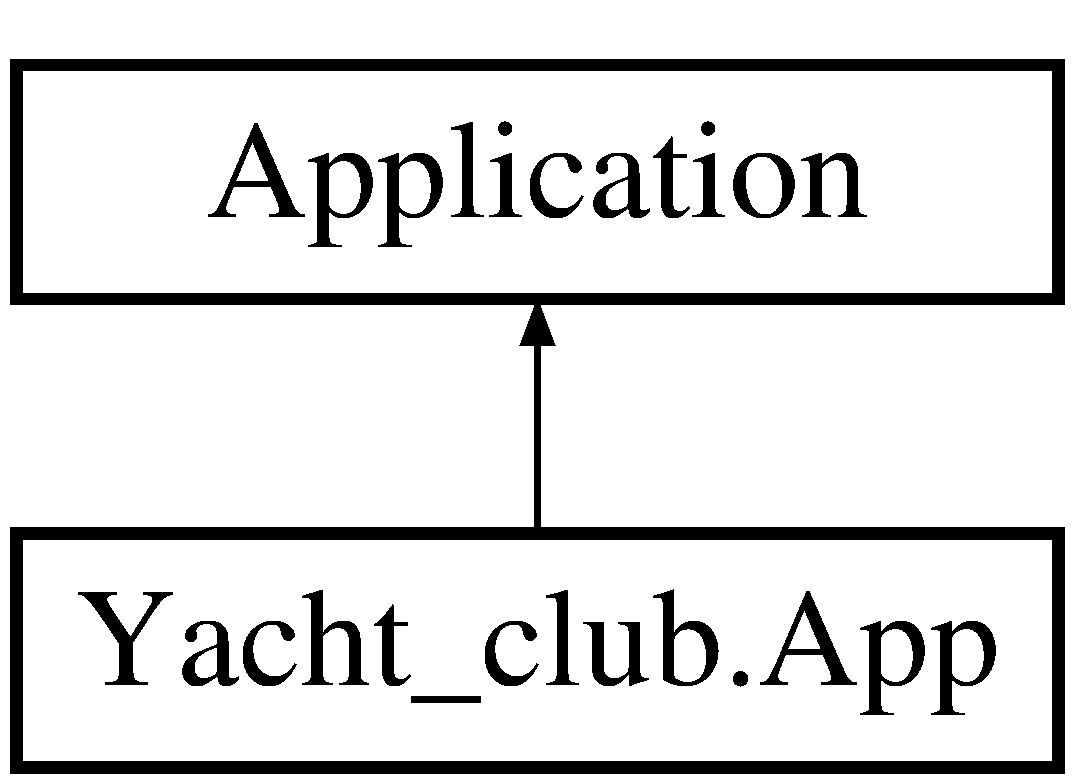
\includegraphics[height=2.000000cm]{class_yacht__club_1_1_app}
\end{center}
\end{figure}


\subsection{Detailed Description}
Interaction logic for App.\+xaml 



The documentation for this class was generated from the following file\+:\begin{DoxyCompactItemize}
\item 
C\+:/\+Users/\+Hikaru/\+Source/\+Repos/Új mappa/trunk/\+Yacht club/\+Yacht club/\textbf{ App.\+xaml.\+cs}\end{DoxyCompactItemize}

\section{Yacht\+\_\+club.\+Main\+\_\+\+Yacht\+\_\+\+Window Class Reference}
\label{class_yacht__club_1_1_main___yacht___window}\index{Yacht\+\_\+club.\+Main\+\_\+\+Yacht\+\_\+\+Window@{Yacht\+\_\+club.\+Main\+\_\+\+Yacht\+\_\+\+Window}}


Interaction logic for Main\+\_\+\+Yacht\+\_\+\+Window.\+xaml  


Inheritance diagram for Yacht\+\_\+club.\+Main\+\_\+\+Yacht\+\_\+\+Window\+:\begin{figure}[H]
\begin{center}
\leavevmode
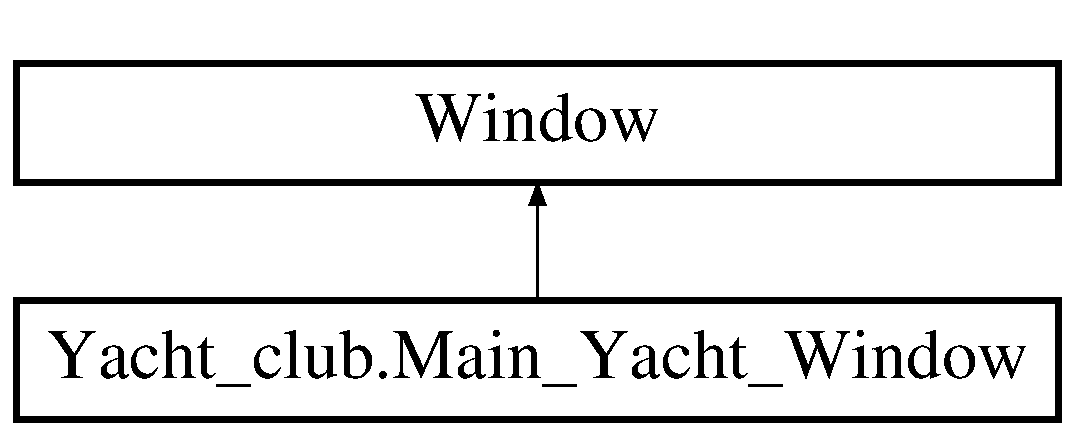
\includegraphics[height=2.000000cm]{class_yacht__club_1_1_main___yacht___window}
\end{center}
\end{figure}
\subsection*{Public Member Functions}
\begin{DoxyCompactItemize}
\item 
void \textbf{ Update\+Theme} ()
\begin{DoxyCompactList}\small\item\em Téma újratöltése a Data\+Context-\/be \end{DoxyCompactList}\item 
\textbf{ Main\+\_\+\+Yacht\+\_\+\+Window} ()
\item 
void \textbf{ log\+Add} (bool Is\+Log)
\begin{DoxyCompactList}\small\item\em Log bejegyzés hozzáadása az egyes usercontrolhoz \end{DoxyCompactList}\end{DoxyCompactItemize}
\subsection*{Protected Member Functions}
\begin{DoxyCompactItemize}
\item 
override void \textbf{ On\+Closed} (Event\+Args e)
\begin{DoxyCompactList}\small\item\em Ez azért kell hogy amikor a login ablak végéez akkor eltünjön \end{DoxyCompactList}\end{DoxyCompactItemize}


\subsection{Detailed Description}
Interaction logic for Main\+\_\+\+Yacht\+\_\+\+Window.\+xaml 



\subsection{Constructor \& Destructor Documentation}
\mbox{\label{class_yacht__club_1_1_main___yacht___window_a87c4e68dfadcb4e53d85a96fd6f8d3b4}} 
\index{Yacht\+\_\+club\+::\+Main\+\_\+\+Yacht\+\_\+\+Window@{Yacht\+\_\+club\+::\+Main\+\_\+\+Yacht\+\_\+\+Window}!Main\+\_\+\+Yacht\+\_\+\+Window@{Main\+\_\+\+Yacht\+\_\+\+Window}}
\index{Main\+\_\+\+Yacht\+\_\+\+Window@{Main\+\_\+\+Yacht\+\_\+\+Window}!Yacht\+\_\+club\+::\+Main\+\_\+\+Yacht\+\_\+\+Window@{Yacht\+\_\+club\+::\+Main\+\_\+\+Yacht\+\_\+\+Window}}
\subsubsection{Main\+\_\+\+Yacht\+\_\+\+Window()}
{\footnotesize\ttfamily Yacht\+\_\+club.\+Main\+\_\+\+Yacht\+\_\+\+Window.\+Main\+\_\+\+Yacht\+\_\+\+Window (\begin{DoxyParamCaption}{ }\end{DoxyParamCaption})}



\subsection{Member Function Documentation}
\mbox{\label{class_yacht__club_1_1_main___yacht___window_a3de96dc62d46d0c97cf6c463742eeae8}} 
\index{Yacht\+\_\+club\+::\+Main\+\_\+\+Yacht\+\_\+\+Window@{Yacht\+\_\+club\+::\+Main\+\_\+\+Yacht\+\_\+\+Window}!log\+Add@{log\+Add}}
\index{log\+Add@{log\+Add}!Yacht\+\_\+club\+::\+Main\+\_\+\+Yacht\+\_\+\+Window@{Yacht\+\_\+club\+::\+Main\+\_\+\+Yacht\+\_\+\+Window}}
\subsubsection{log\+Add()}
{\footnotesize\ttfamily void Yacht\+\_\+club.\+Main\+\_\+\+Yacht\+\_\+\+Window.\+log\+Add (\begin{DoxyParamCaption}\item[{bool}]{Is\+Log }\end{DoxyParamCaption})}



Log bejegyzés hozzáadása az egyes usercontrolhoz 


\begin{DoxyParams}{Parameters}
{\em Is\+Log} & \\
\hline
\end{DoxyParams}
\mbox{\label{class_yacht__club_1_1_main___yacht___window_aba2363333ba6c47878317343c60be7f1}} 
\index{Yacht\+\_\+club\+::\+Main\+\_\+\+Yacht\+\_\+\+Window@{Yacht\+\_\+club\+::\+Main\+\_\+\+Yacht\+\_\+\+Window}!On\+Closed@{On\+Closed}}
\index{On\+Closed@{On\+Closed}!Yacht\+\_\+club\+::\+Main\+\_\+\+Yacht\+\_\+\+Window@{Yacht\+\_\+club\+::\+Main\+\_\+\+Yacht\+\_\+\+Window}}
\subsubsection{On\+Closed()}
{\footnotesize\ttfamily override void Yacht\+\_\+club.\+Main\+\_\+\+Yacht\+\_\+\+Window.\+On\+Closed (\begin{DoxyParamCaption}\item[{Event\+Args}]{e }\end{DoxyParamCaption})\hspace{0.3cm}{\ttfamily [protected]}}



Ez azért kell hogy amikor a login ablak végéez akkor eltünjön 


\begin{DoxyParams}{Parameters}
{\em e} & \\
\hline
\end{DoxyParams}
\mbox{\label{class_yacht__club_1_1_main___yacht___window_a1e7233f8169b3829fe3b06a3733475d1}} 
\index{Yacht\+\_\+club\+::\+Main\+\_\+\+Yacht\+\_\+\+Window@{Yacht\+\_\+club\+::\+Main\+\_\+\+Yacht\+\_\+\+Window}!Update\+Theme@{Update\+Theme}}
\index{Update\+Theme@{Update\+Theme}!Yacht\+\_\+club\+::\+Main\+\_\+\+Yacht\+\_\+\+Window@{Yacht\+\_\+club\+::\+Main\+\_\+\+Yacht\+\_\+\+Window}}
\subsubsection{Update\+Theme()}
{\footnotesize\ttfamily void Yacht\+\_\+club.\+Main\+\_\+\+Yacht\+\_\+\+Window.\+Update\+Theme (\begin{DoxyParamCaption}{ }\end{DoxyParamCaption})}



Téma újratöltése a Data\+Context-\/be 



The documentation for this class was generated from the following file\+:\begin{DoxyCompactItemize}
\item 
C\+:/\+Users/\+Hikaru/\+Source/\+Repos/Új mappa/trunk/\+Yacht club/\+Yacht club/\textbf{ Main\+\_\+\+Yacht\+\_\+\+Window.\+xaml.\+cs}\end{DoxyCompactItemize}

\section{Yacht\+\_\+club.\+w\+Login Class Reference}
\label{class_yacht__club_1_1w_login}\index{Yacht\+\_\+club.\+w\+Login@{Yacht\+\_\+club.\+w\+Login}}


Interaction logic for w\+Login.\+xaml  


Inheritance diagram for Yacht\+\_\+club.\+w\+Login\+:\begin{figure}[H]
\begin{center}
\leavevmode
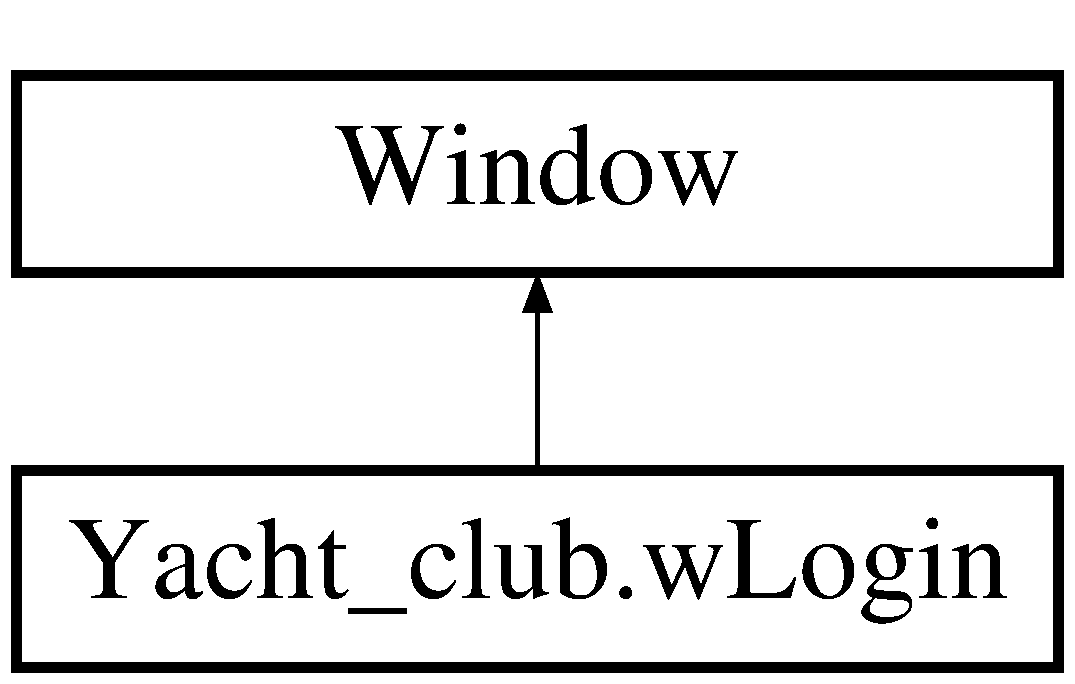
\includegraphics[height=2.000000cm]{class_yacht__club_1_1w_login}
\end{center}
\end{figure}
\subsection*{Public Member Functions}
\begin{DoxyCompactItemize}
\item 
\textbf{ w\+Login} ()
\end{DoxyCompactItemize}
\subsection*{Protected Member Functions}
\begin{DoxyCompactItemize}
\item 
override void \textbf{ On\+Closed} (Event\+Args e)
\end{DoxyCompactItemize}


\subsection{Detailed Description}
Interaction logic for w\+Login.\+xaml 



\subsection{Constructor \& Destructor Documentation}
\mbox{\label{class_yacht__club_1_1w_login_ad570072cc543270f9c8c82c9e210de08}} 
\index{Yacht\+\_\+club\+::w\+Login@{Yacht\+\_\+club\+::w\+Login}!w\+Login@{w\+Login}}
\index{w\+Login@{w\+Login}!Yacht\+\_\+club\+::w\+Login@{Yacht\+\_\+club\+::w\+Login}}
\subsubsection{w\+Login()}
{\footnotesize\ttfamily Yacht\+\_\+club.\+w\+Login.\+w\+Login (\begin{DoxyParamCaption}{ }\end{DoxyParamCaption})}



\subsection{Member Function Documentation}
\mbox{\label{class_yacht__club_1_1w_login_a9a623be68725f0b0b1f3c86255891a81}} 
\index{Yacht\+\_\+club\+::w\+Login@{Yacht\+\_\+club\+::w\+Login}!On\+Closed@{On\+Closed}}
\index{On\+Closed@{On\+Closed}!Yacht\+\_\+club\+::w\+Login@{Yacht\+\_\+club\+::w\+Login}}
\subsubsection{On\+Closed()}
{\footnotesize\ttfamily override void Yacht\+\_\+club.\+w\+Login.\+On\+Closed (\begin{DoxyParamCaption}\item[{Event\+Args}]{e }\end{DoxyParamCaption})\hspace{0.3cm}{\ttfamily [protected]}}



The documentation for this class was generated from the following file\+:\begin{DoxyCompactItemize}
\item 
C\+:/\+Users/\+Hikaru/\+Source/\+Repos/Új mappa/trunk/\+Yacht club/\+Yacht club/\textbf{ w\+Login.\+xaml.\+cs}\end{DoxyCompactItemize}

\section{Yacht\+\_\+club.\+w\+Message Class Reference}
\label{class_yacht__club_1_1w_message}\index{Yacht\+\_\+club.\+w\+Message@{Yacht\+\_\+club.\+w\+Message}}


Interaction logic for w\+Message.\+xaml  


Inheritance diagram for Yacht\+\_\+club.\+w\+Message\+:\begin{figure}[H]
\begin{center}
\leavevmode
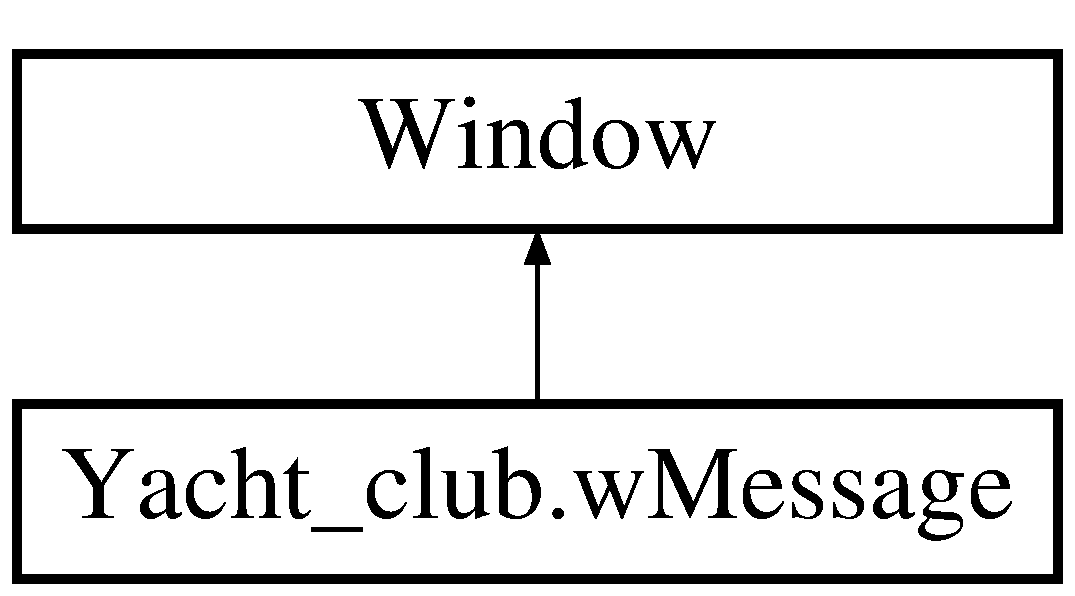
\includegraphics[height=2.000000cm]{class_yacht__club_1_1w_message}
\end{center}
\end{figure}
\subsection*{Public Member Functions}
\begin{DoxyCompactItemize}
\item 
\textbf{ w\+Message} (int action, int id)
\begin{DoxyCompactList}\small\item\em Az akció id-\/je és a folyamathoz szükséged id eltárolása \end{DoxyCompactList}\end{DoxyCompactItemize}


\subsection{Detailed Description}
Interaction logic for w\+Message.\+xaml 



\subsection{Constructor \& Destructor Documentation}
\mbox{\label{class_yacht__club_1_1w_message_a92d68bf00eddabe763512d315981e0e2}} 
\index{Yacht\+\_\+club\+::w\+Message@{Yacht\+\_\+club\+::w\+Message}!w\+Message@{w\+Message}}
\index{w\+Message@{w\+Message}!Yacht\+\_\+club\+::w\+Message@{Yacht\+\_\+club\+::w\+Message}}
\subsubsection{w\+Message()}
{\footnotesize\ttfamily Yacht\+\_\+club.\+w\+Message.\+w\+Message (\begin{DoxyParamCaption}\item[{int}]{action,  }\item[{int}]{id }\end{DoxyParamCaption})}



Az akció id-\/je és a folyamathoz szükséged id eltárolása 


\begin{DoxyParams}{Parameters}
{\em action} & ablak akció id\\
\hline
{\em id} & folyamat id\\
\hline
\end{DoxyParams}


The documentation for this class was generated from the following file\+:\begin{DoxyCompactItemize}
\item 
C\+:/\+Users/\+Hikaru/\+Source/\+Repos/Új mappa/trunk/\+Yacht club/\+Yacht club/\textbf{ w\+Message.\+xaml.\+cs}\end{DoxyCompactItemize}

\chapter{File Documentation}
\section{C\+:/\+Users/\+Hikaru/\+Source/\+Repos/Új mappa/trunk/\+Yacht club/\+Yacht club/\+App.xaml.\+cs File Reference}
\label{_app_8xaml_8cs}\index{C\+:/\+Users/\+Hikaru/\+Source/\+Repos/Új mappa/trunk/\+Yacht club/\+Yacht club/\+App.\+xaml.\+cs@{C\+:/\+Users/\+Hikaru/\+Source/\+Repos/Új mappa/trunk/\+Yacht club/\+Yacht club/\+App.\+xaml.\+cs}}
\subsection*{Classes}
\begin{DoxyCompactItemize}
\item 
class \textbf{ Yacht\+\_\+club.\+App}
\begin{DoxyCompactList}\small\item\em Interaction logic for App.\+xaml \end{DoxyCompactList}\end{DoxyCompactItemize}
\subsection*{Namespaces}
\begin{DoxyCompactItemize}
\item 
namespace \textbf{ Yacht\+\_\+club}
\end{DoxyCompactItemize}

\section{C\+:/\+Users/\+Hikaru/\+Source/\+Repos/Új mappa/trunk/\+Yacht club/\+Yacht club/\+Main\+\_\+\+Yacht\+\_\+\+Window.xaml.\+cs File Reference}
\label{_main___yacht___window_8xaml_8cs}\index{C\+:/\+Users/\+Hikaru/\+Source/\+Repos/Új mappa/trunk/\+Yacht club/\+Yacht club/\+Main\+\_\+\+Yacht\+\_\+\+Window.\+xaml.\+cs@{C\+:/\+Users/\+Hikaru/\+Source/\+Repos/Új mappa/trunk/\+Yacht club/\+Yacht club/\+Main\+\_\+\+Yacht\+\_\+\+Window.\+xaml.\+cs}}
\subsection*{Classes}
\begin{DoxyCompactItemize}
\item 
class \textbf{ Yacht\+\_\+club.\+Main\+\_\+\+Yacht\+\_\+\+Window}
\begin{DoxyCompactList}\small\item\em Interaction logic for Main\+\_\+\+Yacht\+\_\+\+Window.\+xaml \end{DoxyCompactList}\end{DoxyCompactItemize}
\subsection*{Namespaces}
\begin{DoxyCompactItemize}
\item 
namespace \textbf{ Yacht\+\_\+club}
\end{DoxyCompactItemize}

\section{C\+:/\+Users/\+Hikaru/\+Source/\+Repos/Új mappa/trunk/\+Yacht club/\+Yacht club/w\+Login.xaml.\+cs File Reference}
\label{w_login_8xaml_8cs}\index{C\+:/\+Users/\+Hikaru/\+Source/\+Repos/Új mappa/trunk/\+Yacht club/\+Yacht club/w\+Login.\+xaml.\+cs@{C\+:/\+Users/\+Hikaru/\+Source/\+Repos/Új mappa/trunk/\+Yacht club/\+Yacht club/w\+Login.\+xaml.\+cs}}
\subsection*{Classes}
\begin{DoxyCompactItemize}
\item 
class \textbf{ Yacht\+\_\+club.\+w\+Login}
\begin{DoxyCompactList}\small\item\em Interaction logic for w\+Login.\+xaml \end{DoxyCompactList}\end{DoxyCompactItemize}
\subsection*{Namespaces}
\begin{DoxyCompactItemize}
\item 
namespace \textbf{ Yacht\+\_\+club}
\end{DoxyCompactItemize}

\section{C\+:/\+Users/\+Hikaru/\+Source/\+Repos/Új mappa/trunk/\+Yacht club/\+Yacht club/w\+Message.xaml.\+cs File Reference}
\label{w_message_8xaml_8cs}\index{C\+:/\+Users/\+Hikaru/\+Source/\+Repos/Új mappa/trunk/\+Yacht club/\+Yacht club/w\+Message.\+xaml.\+cs@{C\+:/\+Users/\+Hikaru/\+Source/\+Repos/Új mappa/trunk/\+Yacht club/\+Yacht club/w\+Message.\+xaml.\+cs}}
\subsection*{Classes}
\begin{DoxyCompactItemize}
\item 
class \textbf{ Yacht\+\_\+club.\+w\+Message}
\begin{DoxyCompactList}\small\item\em Interaction logic for w\+Message.\+xaml \end{DoxyCompactList}\end{DoxyCompactItemize}
\subsection*{Namespaces}
\begin{DoxyCompactItemize}
\item 
namespace \textbf{ Yacht\+\_\+club}
\end{DoxyCompactItemize}

%--- End generated contents ---

% Index
\backmatter
\newpage
\phantomsection
\clearemptydoublepage
\addcontentsline{toc}{chapter}{Index}
\printindex

\end{document}
